\section{Fonctions, la pile et la libC}
The machine has no notion of a function. It has registres, a flat array of bytes
and a program counter, and that is all. Everything that makes a function ---
parameters, local variables, a valeur de retour, the guarantee that the
appelant's data survives the call --- is an agreement between two pieces of code
that never meet. This chapter states that agreement. It begins with the memory a
processus is given, narrows to the region that agreement lives in (the pile),
then fixes the System V calling convention that \texttt{gcc} and the libC both
obey, and ends by calling \texttt{scanf} and \texttt{printf} from bare assembly.

\subsection{Organisation de la mémoire}
\begin{definition}[Les trois parties de la mémoire d'un programme]
  En simplifiant beaucoup, la mémoire d'un programme est composée de trois
  parties :
  \begin{itemize}
    \item la \textbf{mémoire statique} (\textit{static memory}) chargée par l'OS
      depuis l'ELF (le contenu des sections \texttt{.text}, \texttt{.data},
      \texttt{.bss}, etc.) ;
    \item la \textbf{pile} (\textit{stack}), qui est une mémoire fournie par
      l'OS \emph{pour les fonctions} ; l'OS fournit directement cette mémoire ;
    \item le \textbf{tas} (\textit{heap}), qui est une mémoire fournie par l'OS
      \emph{sur demande}.
  \end{itemize}
\end{definition}

The distinction that matters for this chapter is the second one. The mémoire
statique is fixed at the édition de liens and the tas has to be requested
(through \texttt{malloc}, i.e.\ ultimately through a system call); the pile is
simply \emph{there} when the processus starts, without being asked for, which is
why a function can allocate its working space in a single subtraction and free
it in a single addition.

\begin{figure}[h!]
  \centering
  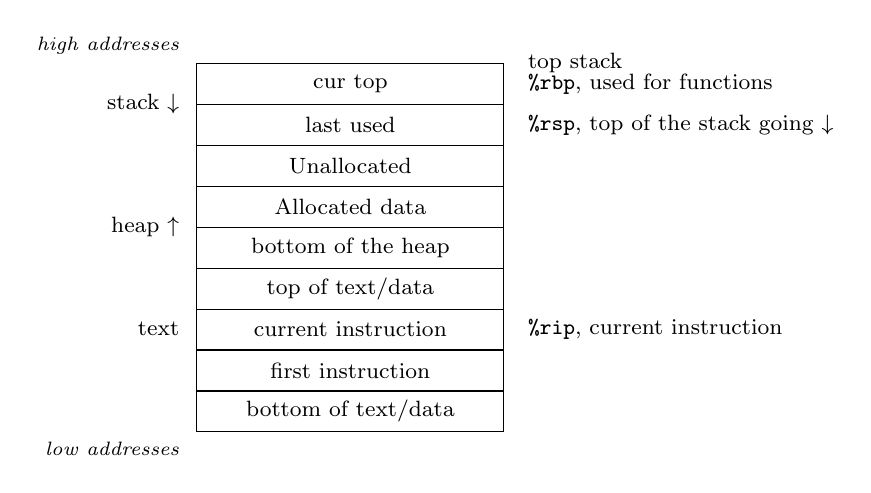
\begin{tikzpicture}[font=\footnotesize]
    \tikzset{
      cell/.style={draw, minimum width=3.9cm, minimum height=0.52cm,
                   inner sep=1pt, anchor=north},
      ann/.style={anchor=west, xshift=5pt},
    }
    \node[cell] (ra) at (0, 0.00) {cur top};
    \node[cell] (rb) at (0,-0.52) {last used};
    \node[cell] (rc) at (0,-1.04) {Unallocated};
    \node[cell] (rd) at (0,-1.56) {Allocated data};
    \node[cell] (re) at (0,-2.08) {bottom of the heap};
    \node[cell] (rf) at (0,-2.60) {top of text/data};
    \node[cell] (rg) at (0,-3.12) {current instruction};
    \node[cell] (rh) at (0,-3.64) {first instruction};
    \node[cell] (ri) at (0,-4.16) {bottom of text/data};

    \node[ann] at (ra.north east) {top stack};
    \node[ann] at (ra.east) {\texttt{\%rbp}, used for functions};
    \node[ann] at (rb.east) {\texttt{\%rsp}, top of the stack going $\downarrow$};
    \node[ann] at (rg.east) {\texttt{\%rip}, current instruction};

    \node[anchor=east] at (-2.05,-0.52) {stack $\downarrow$};
    \node[anchor=east] at (-2.05,-2.08) {heap $\uparrow$};
    \node[anchor=east] at (-2.05,-3.38) {text};

    \node[anchor=east, font=\scriptsize\itshape] at (-2.05, 0.22) {high addresses};
    \node[anchor=east, font=\scriptsize\itshape] at (-2.05,-4.90) {low addresses};
  \end{tikzpicture}
\end{figure}

Read the picture from the bottom: the text and data loaded from the ELF sit at
the low addresses, the tas grows \emph{upwards} from just above them, and the
pile grows \emph{downwards} from the top. Between the two lies unallocated
address space, which is what lets both grow. Three registres point into this
picture: \texttt{\%rip} into the text at the current instruction, \texttt{\%rsp}
at the top of the pile, and \texttt{\%rbp} somewhat higher up in the pile,
``used for functions''.

\subsubsection{Organisation de la pile pour les fonctions}
\begin{definition}[Organisation de la pile pour les fonctions (\textit{stack discipline})]
  Il est \emph{standard} --- not enforced by the hardware --- que :
  \begin{itemize}
    \item \textbf{presque toujours}, \texttt{\%rsp} pointe vers le premier
      octet utilisé de la pile ;
    \item \textbf{souvent} \texttt{\%rbp} pointe vers le début de la pile au
      début de l'appel de la fonction courante.
  \end{itemize}
\end{definition}

\begin{remark}
  The hedging is worth keeping. ``Presque toujours'' and ``souvent'' are the
  right words because nothing in the processor checks either claim:
  \texttt{\%rsp} and \texttt{\%rbp} are ordinary registres généraux. Only the
  instructions \texttt{push}, \texttt{pop}, \texttt{call} and \texttt{ret} ---
  and the interrupt machinery --- treat \texttt{\%rsp} specially.
  \texttt{\%rbp} is special to nobody at all; it is a convention kept by
  compilateurs.
\end{remark}

\paragraph{Manipuler la pile}
Les commandes suivantes permettent de manipuler la pile :
\begin{itemize}
  \item \texttt{push \%rbx} ou \texttt{pushq \$42} décale \texttt{\%rsp} de la
    bonne taille puis stocke \texttt{\%rbx}/\texttt{42} dans \texttt{(\%rsp)} ;
  \item \texttt{pop \%rbx} récupère la valeur \texttt{(\%rsp)} dans
    \texttt{\%rbx} puis décale \texttt{\%rsp} de la bonne taille.
\end{itemize}
Ces commandes peuvent s'écrire autrement (\texttt{add} + \texttt{mov}). Since
the pile grows towards the low addresses, ``décale \texttt{\%rsp} de la bonne
taille'' means \emph{subtracting} the operand size on a push and \emph{adding}
it on a pop:

\begin{lstlisting}[language=gas]
        pushq   %rbx            # is the pair
        subq    $8, %rsp
        movq    %rbx, (%rsp)

        popq    %rbx            # is the pair
        movq    (%rsp), %rbx
        addq    $8, %rsp
\end{lstlisting}

\begin{remark}
  Note the order inside each pair: a push decrements \emph{then} writes, a pop
  reads \emph{then} increments. \texttt{(\%rsp)} therefore always denotes a byte
  that is in use, never free space. Note also that the two halves are ordinary
  instructions, so nothing stops you from moving \texttt{\%rsp} by hand:
  \texttt{subq \$32, \%rsp} allocates thirty-two bytes in one stroke, which is
  exactly what a function prologue does, and is far cheaper than four pushes.
\end{remark}

\subsection{Fonctions en assembleur}
\begin{definition}[Les fonctions ne sont que des conventions]
  \emph{En assembleur les fonctions ne sont que des conventions.} In assembly a
  function is not a language construct; it is a pair of promises, one kept by
  the code that calls, the \textbf{appelant} (\textit{caller}), and one kept by
  the code that is called, the \textbf{fonction appelée} (\textit{callee}), about
  where arguments live, where the result is left, which registres survive, and
  where execution resumes.
\end{definition}

\subsubsection{L'appelant}
Avant d'appeler une fonction, \texttt{gcc} va :
\begin{itemize}
  \item sauvegarder les registres que la fonction appelée risque d'écraser ;
  \item stocker les arguments à des endroits prédéfinis (p.~ex.\ sur les
    registres puis la pile) ;
  \item stocker l'adresse de l'instruction à exécuter une fois que la fonction
    termine ;
  \item sauter au début de la fonction ;
  \item en revenant, retirer les arguments mis sur la pile ;
  \item restaurer la valeur des registres sauvegardés.
\end{itemize}
The third and fourth steps together are precisely what the \texttt{call}
instruction does; the rest is code the compilateur emits around it.

\subsubsection{La fonction appelée}
Pour une fonction appelée, \texttt{gcc} va :
\begin{itemize}
  \item allouer une \textbf{frame} et sauvegarder le \texttt{\%rbp} précédent ;
  \item faire le calcul ;
  \item libérer la frame ;
  \item revenir à l'appelant.
\end{itemize}
The first item is the \textbf{prologue}, the last two the \textbf{epilogue}.

\subsubsection{Quelques commandes utiles pour les fonctions}
\begin{center}
  \begin{tabularx}{\textwidth}{lX}
    \toprule
    instruction & effect \\
    \midrule
    \texttt{call label} &
      plus ou moins équivalent à \texttt{push \%rip+8} combiné à
      \texttt{jmp label} \\
    \texttt{ret} &
      plus ou moins équivalent à \texttt{pop \%rip} \\
    \texttt{enter 32} &
      équivalent à \texttt{pushq \%rbp}, \texttt{movq \%rsp, \%rbp},
      \texttt{subq \$32, \%rsp}, mais n'est généralement pas utilisé \\
    \texttt{leave} &
      équivalent à \texttt{movq \%rbp, \%rsp}, \texttt{pop \%rbp}, un peu plus
      souvent utilisé \\
    \bottomrule
  \end{tabularx}
\end{center}

\begin{remark}
  The ``plus ou moins'' in the first two rows is essential. \texttt{\%rip} is not
  an addressable registre général on x86-64: \texttt{push \%rip} and
  \texttt{pop \%rip} are not instructions you can assemble. The equivalence
  describes the \emph{effect} --- \texttt{call} pushes the return address and
  transfers control, \texttt{ret} pops it back into the program counter --- not
  a rewriting you may type. The \texttt{+8} likewise stands for ``the length of
  the \texttt{call} instruction''; what is pushed is the address of the
  instruction that follows the \texttt{call}.
\end{remark}

\begin{remark}
  \texttt{enter} and \texttt{leave} are single instructions that package a
  whole prologue and epilogue. \texttt{enter} is slow enough on modern
  processors that compilateurs avoid it; \texttt{leave} survives because it is
  one byte and does exactly the right thing.
\end{remark}

\subsubsection{La frame}
The standard prologue and epilogue, written out longhand, are
\begin{lstlisting}[language=gas]
f:      pushq   %rbp            # save the caller's frame pointer
        movq    %rsp, %rbp      # this frame starts here
        subq    $32, %rsp       # 32 bytes of local variables
        # ... the computation ...
        movq    %rbp, %rsp      # free the frame  (these two lines = leave)
        popq    %rbp
        ret
\end{lstlisting}
so that \texttt{enter 32} replaces the first three lines and \texttt{leave}
replaces the two that free the frame.

\begin{figure}[h!]
  \centering
  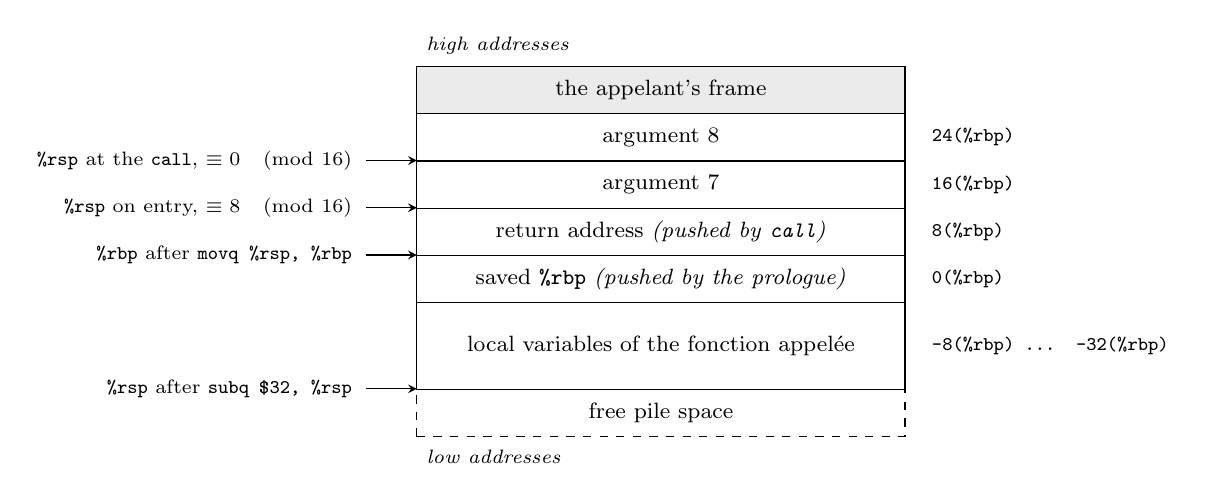
\begin{tikzpicture}[font=\footnotesize, >=stealth]
    \tikzset{
      cell/.style={draw, minimum width=6.2cm, inner sep=2pt, anchor=north},
      lab/.style={anchor=east, font=\scriptsize},
      off/.style={anchor=west, xshift=6pt, font=\scriptsize\ttfamily},
    }
    \node[cell, minimum height=0.6cm, fill=black!8] (c0) at (0, 0.00) {the appelant's frame};
    \node[cell, minimum height=0.6cm] (c1) at (0,-0.60) {argument 8};
    \node[cell, minimum height=0.6cm] (c2) at (0,-1.20) {argument 7};
    \node[cell, minimum height=0.6cm] (c3) at (0,-1.80) {return address \emph{(pushed by \texttt{call})}};
    \node[cell, minimum height=0.6cm] (c4) at (0,-2.40) {saved \texttt{\%rbp} \emph{(pushed by the prologue)}};
    \node[cell, minimum height=1.1cm] (c5) at (0,-3.00) {local variables of the fonction appelée};
    \node[cell, minimum height=0.6cm, dashed] (c6) at (0,-4.10) {free pile space};

    \node[off] at (c1.east) {24(\%rbp)};
    \node[off] at (c2.east) {16(\%rbp)};
    \node[off] at (c3.east) {8(\%rbp)};
    \node[off] at (c4.east) {0(\%rbp)};
    \node[off] at (c5.east) {-8(\%rbp) ... -32(\%rbp)};

    \draw[->] (-3.75,-1.20) -- (-3.10,-1.20);
    \node[lab] at (-3.80,-1.20) {\texttt{\%rsp} at the \texttt{call}, $\equiv 0 \pmod{16}$};
    \draw[->] (-3.75,-1.80) -- (-3.10,-1.80);
    \node[lab] at (-3.80,-1.80) {\texttt{\%rsp} on entry, $\equiv 8 \pmod{16}$};
    \draw[->] (-3.75,-2.40) -- (-3.10,-2.40);
    \node[lab] at (-3.80,-2.40) {\texttt{\%rbp} after \texttt{movq \%rsp, \%rbp}};
    \draw[->] (-3.75,-4.10) -- (-3.10,-4.10);
    \node[lab] at (-3.80,-4.10) {\texttt{\%rsp} after \texttt{subq \$32, \%rsp}};

    \node[anchor=west, font=\scriptsize\itshape] at (-3.10, 0.26) {high addresses};
    \node[anchor=west, font=\scriptsize\itshape] at (-3.10,-4.96) {low addresses};
  \end{tikzpicture}
\end{figure}

Once \texttt{\%rbp} has been set, every interesting slot has a fixed offset from
it, and those offsets stay valid no matter how much \texttt{\%rsp} subsequently
moves. That is the whole point of keeping a pointeur to the frame:
\texttt{0(\%rbp)} holds the appelant's saved \texttt{\%rbp}, \texttt{8(\%rbp)}
the return address,
\texttt{16(\%rbp)} the seventh argument if there is one, and the local variables
live at the negative offsets \texttt{-8(\%rbp)}, \texttt{-16(\%rbp)} and so on.
Addressing the same locals off \texttt{\%rsp} would require recomputing every
offset after each push.

\subsection{La convention d'appel}
The ``endroits prédéfinis'' of the appelant's second step are not a free choice.
On Linux they are fixed by the \textbf{System V AMD64 ABI}, which is the
convention \texttt{gcc} emits and the libC expects. Assembly that calls the libC
must obey it exactly; assembly that only calls itself may do as it pleases, but
there is no reason to invent a second convention. Naming the ABI and its
registres goes beyond this course, which says only that the arguments are stored
\textit{à des endroits prédéfinis} and that one must make \textit{des appels
alignés sur des multiples de 16}. This subsection fills those two phrases in
from the ABI itself.

\subsubsection{Où vont les arguments}
\begin{definition}[Registres d'argument (\textit{argument registers}), dans l'ordre]
  Arguments that are integers or pointeurs are passed in the registres
  \[
    \texttt{\%rdi},\quad \texttt{\%rsi},\quad \texttt{\%rdx},\quad
    \texttt{\%rcx},\quad \texttt{\%r8},\quad \texttt{\%r9}
  \]
  in that order; the seventh and later integer arguments are pushed on the
  pile. Floating-point arguments go in \texttt{\%xmm0} through
  \texttt{\%xmm7}. The two sequences are consumed independently.
\end{definition}

\begin{center}
  \begin{tabular}{lcccccccc}
    \toprule
    argument $n$ & 1 & 2 & 3 & 4 & 5 & 6 & 7 & 8 \\
    \midrule
    integer / pointeur &
      \texttt{\%rdi} & \texttt{\%rsi} & \texttt{\%rdx} & \texttt{\%rcx} &
      \texttt{\%r8} & \texttt{\%r9} & pile & pile \\
    floating point &
      \texttt{\%xmm0} & \texttt{\%xmm1} & \texttt{\%xmm2} & \texttt{\%xmm3} &
      \texttt{\%xmm4} & \texttt{\%xmm5} & \texttt{\%xmm6} & \texttt{\%xmm7} \\
    \bottomrule
  \end{tabular}
\end{center}

The arguments passed on the pile are laid out so that the seventh sits at the
\emph{lowest} address, that is, at \texttt{(\%rsp)} at the instant the
\texttt{call} executes, the eighth at \texttt{8(\%rsp)}, and so on. They are the
appelant's property: removing them after the call is the appelant's fifth step,
and it is one addition to \texttt{\%rsp}.

\begin{definition}[Valeur de retour (\textit{return value})]
  The result comes back in \texttt{\%rax} (in the pair
  \texttt{\%rdx}:\texttt{\%rax} for a 128-bit value) for integers and pointeurs,
  and in \texttt{\%xmm0} for floating point.
\end{definition}

\begin{definition}[\texttt{\%al} et fonctions variadiques]
  For a \textbf{fonction variadique} (\textit{variadic function}) --- one
  declared with \texttt{\dots}, such as \texttt{printf} and \texttt{scanf} ---
  the appelant must additionally set \texttt{\%al} to the number of vector
  (\texttt{\%xmm}) registres used to pass arguments.
\end{definition}

This is what the line \texttt{mov \$0, \%rax} does in every libC example below.
It is not decoration and it is not a cleared valeur de retour: it announces ``no
floating-point argument was passed''. A fonction variadique uses the count to
decide whether it must spill the eight \texttt{\%xmm} registres into its save
area for registres; leaving \texttt{\%rax} holding garbage makes \texttt{printf}
read vector registres it was never given, and the call may fault.

\subsubsection{Questions d'alignement}
\begin{definition}[Alignement (\textit{alignment}) naturel]
  Quand on lit un bloc de taille $2^{k}$, le processeur s'attend à ce que
  l'adresse lue soit un multiple de $2^{k}$.
\end{definition}
Pour \texttt{movq}, \texttt{movl}, \texttt{movw}, \texttt{movb} et toutes les
instructions vues jusqu'à présent ce n'est pas un problème, mais il existe des
instructions qui \emph{s'attendent} à des adresses alignées. x86 tolerates
misaligned ordinary loads and stores, at a speed penalty; the instructions that
expect aligned addresses fault otherwise. Même si vos instructions ignorent
l'alignement, la libC peut l'attendre, il faut donc faire des appels alignés sur
des multiples de $16$.

\begin{definition}[La règle des 16 octets avant un \texttt{call}]
  At the instant the \texttt{call} instruction executes, \texttt{\%rsp} must be
  a multiple of $16$. Since \texttt{call} then pushes an eight-byte return
  address, on entry to the fonction appelée
  \[
    \texttt{\%rsp} \equiv 8 \pmod{16},
  \]
  and the fonction appelée's own \texttt{pushq \%rbp} brings it back to a
  multiple of $16$.
\end{definition}

\begin{figure}[h!]
  \centering
  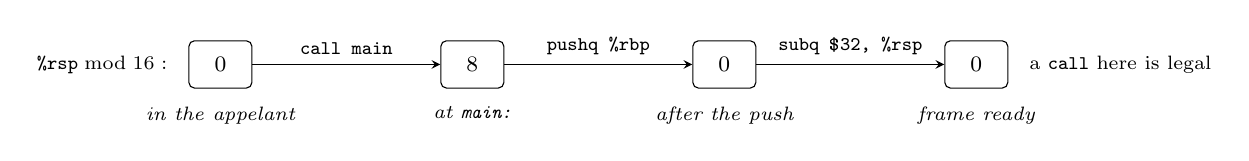
\begin{tikzpicture}[font=\footnotesize, >=stealth]
    \tikzset{
      st/.style={draw, rounded corners=2pt, minimum width=0.8cm,
                 minimum height=0.6cm, inner sep=2pt},
      op/.style={above, font=\scriptsize\ttfamily},
      frmcap/.style={below=3pt, font=\scriptsize\itshape},
    }
    \node[st] (A) at (0.0,0) {$0$};
    \node[st] (B) at (3.2,0) {$8$};
    \node[st] (C) at (6.4,0) {$0$};
    \node[st] (D) at (9.6,0) {$0$};

    \draw[->] (A) -- node[op]{call main} (B);
    \draw[->] (B) -- node[op]{pushq \%rbp} (C);
    \draw[->] (C) -- node[op]{subq \$32, \%rsp} (D);

    \node[frmcap] at (A.south) {in the appelant};
    \node[frmcap] at (B.south) {at \texttt{main:}};
    \node[frmcap] at (C.south) {after the push};
    \node[frmcap] at (D.south) {frame ready};

    \node[anchor=east, font=\scriptsize] at (-0.55,0) {$\texttt{\%rsp} \bmod 16:$};
    \node[anchor=west, font=\scriptsize] at (10.15,0) {a \texttt{call} here is legal};
  \end{tikzpicture}
\end{figure}

\begin{remark}
  Two corollaries that the exercises trip over. First, the frame size must be a
  multiple of $16$: after the entry offset of $8$ and the eight-byte
  \texttt{pushq \%rbp}, \texttt{subq \$32, \%rsp} preserves the alignement
  because $32 \equiv 0 \pmod{16}$, whereas \texttt{subq \$24, \%rsp} would
  destroy it and the next \texttt{call printf} would be misaligned. This is the
  meaning of the warning \textit{``attention gcc peut attendre un alignement 16
  octets''} in the libC skeleton below. Second, an odd number of pushes leaves
  the pile misaligned, so a function that pushes three registres sauvegardés par
  l'appelé must push a fourth value --- or subtract eight --- before it may call
  anything.
\end{remark}

\begin{remark}
  The ABI also reserves the $128$ bytes immediately below \texttt{\%rsp} as the
  \textbf{zone rouge} (\textit{red zone}), which a leaf function may scribble on
  without moving \texttt{\%rsp} at all. It goes beyond this course, and it is
  unusable in any function that makes a call, since the \texttt{call} itself
  overwrites the top of it.
\end{remark}

\subsubsection{Registres sauvegardés par l'appelant et par l'appelé}
The appelant's first and last steps --- \textit{sauvegarder les registres que la
fonction appelée risque d'écraser}, then \textit{restaurer la valeur des
registres sauvegardés} --- raise the obvious question of which registres those
are. The convention answers it by splitting the set of registres in two.

\begin{center}
  \begin{tabularx}{\textwidth}{lX}
    \toprule
    \textbf{sauvegardés par l'appelant}, volatile &
      \texttt{\%rax}, \texttt{\%rcx}, \texttt{\%rdx}, \texttt{\%rsi},
      \texttt{\%rdi}, \texttt{\%r8}--\texttt{\%r11}, and all the
      \texttt{\%xmm} registres \\
    \addlinespace
    \textbf{sauvegardés par l'appelé}, non-volatile &
      \texttt{\%rbx}, \texttt{\%rbp}, \texttt{\%rsp},
      \texttt{\%r12}--\texttt{\%r15} \\
    \bottomrule
  \end{tabularx}
\end{center}

\begin{definition}[Les deux promesses]
  A registre \textbf{sauvegardé par l'appelant} (\textit{caller-saved}) may be
  destroyed freely by the fonction appelée; if the appelant still needs its
  value after the call, the appelant must save it. A registre
  \textbf{sauvegardé par l'appelé} (\textit{callee-saved}) must have the same
  value when the function returns as it had on entry; if the fonction appelée
  wants to use it, the fonction appelée must push it in its prologue and pop it
  in its epilogue.
\end{definition}

\begin{remark}
  No registre is intrinsically ``safe''. The split only says \emph{who pays}. It
  is chosen so that the registres d'argument and the scratch registres are
  volatile --- an appelant that has already consumed its arguments loses nothing
  by them being clobbered --- while a fonction appelée that wants a long-lived
  value has \texttt{\%rbx} and \texttt{\%r12}--\texttt{\%r15} available at the
  price of one push each.
\end{remark}

\begin{remark}
  The fonction appelée's first step, ``allouer une frame et sauvegarder le
  \texttt{\%rbp} précédent'', is nothing other than \texttt{\%rbp} being
  sauvegardé par l'appelé, and \texttt{\%rsp} appears in the sauvegardés par
  l'appelé row for the same reason: the epilogue must hand \texttt{\%rsp} back
  exactly where it found it, or \texttt{ret} will pop the wrong word.
\end{remark}

\subsection{Utiliser la libC}
\subsubsection{Schéma général}
\begin{lstlisting}[language=gas]
        .data

        .text
        .globl main
main:   ; main est une fonction, on doit ret
        push %rbp
        movq %rsp, %rbp
        subq $32, %rsp ; attention gcc peut attendre
        ; un alignement 16 octets

        ret
        .section .note.GNU-stack
\end{lstlisting}

Three things in this skeleton are not optional. The global symbol is
\texttt{main} and not \texttt{\_start}: the édition de liens against the libC
brings in its startup code, which runs first, initialises the library and then
\emph{calls} \texttt{main}. \texttt{main} is therefore an ordinary function and
must \texttt{ret} --- as the comment in the listing says, \textit{main est une
fonction, on doit ret} --- returning its exit status in \texttt{\%eax}. Falling
off the end, or ending with an \texttt{exit} system call, would skip the
library's own shutdown.

\begin{remark}
  The final line \texttt{.section .note.GNU-stack} emits the empty note section
  by which a fichier objet declares that it does not need an executable pile. It
  carries no code; without it the linker assumes the worst and warns.
\end{remark}

\begin{remark}
  The frame here is thirty-two bytes and the comment on the \texttt{subq} flags
  exactly the trap of the previous subsection: a size that is not a multiple of
  sixteen leaves \texttt{\%rsp} misaligned for every subsequent call into the
  libC.
\end{remark}

\begin{remark}
  The skeleton is nevertheless incomplete as printed: it allocates the frame and
  never frees it. Between \texttt{subq \$32, \%rsp} and \texttt{ret} it has no
  \texttt{leave} and no \texttt{movq \%rbp, \%rsp} followed by
  \texttt{popq \%rbp}, so at the \texttt{ret} \texttt{\%rsp} still sits
  thirty-two bytes below the saved \texttt{\%rbp}: \texttt{ret} pops a local
  variable rather than the return address, and control jumps to garbage. The
  blank line is where the body goes, and the epilogue written longhand above ---
  \texttt{movq \%rbp, \%rsp} then \texttt{popq \%rbp}, or simply \texttt{leave}
  --- belongs immediately before the \texttt{ret}.
\end{remark}

\subsubsection{\texttt{scanf}}
\begin{lstlisting}[language=gas]
        .data
int_fmt:
        .string "%d" ; pour scanf, c'est un entier
        .text
        .globl main
main: ; main est une fonction, on doit ret
        pushq   $0 ; on alloue un espace sur la stack
        leaq    (%rsp), %rsi ; on met l'adresse dans %rsi
        leaq    int_fmt(%rip), %rdi ; format dans %rdi
        mov     $0, %rax ; on met 0 dans rax
        call    scanf
        popq    %rax
        ret
        .section .note.GNU-stack
\end{lstlisting}

Line by line, against the convention just stated:
\begin{itemize}
  \item \texttt{pushq \$0} allocates eight zeroed bytes on the pile. It does
    double duty: it is the storage \texttt{scanf} will write into, \emph{and} it
    moves \texttt{\%rsp} from $\equiv 8$ back to $\equiv 0 \pmod{16}$, so the
    coming \texttt{call} is aligned.
  \item \texttt{leaq (\%rsp), \%rsi} puts the \emph{address} of that slot into
    the second registre d'argument. \texttt{scanf} wants somewhere to store, so
    it takes a pointeur --- this is why the C call is \texttt{scanf("\%d", \&n)}.
  \item \texttt{leaq int\_fmt(\%rip), \%rdi} puts the address of the format, a
    chaîne de caractères, into the first registre d'argument.
  \item \texttt{mov \$0, \%rax} declares zero vector registres used, as every
    variadic call must.
  \item \texttt{popq \%rax} frees the slot --- and, as a bonus, leaves the value
    that was read in \texttt{\%rax}.
\end{itemize}

\begin{remark}[\texttt{\%rip}-relative addressing]
  \texttt{leaq int\_fmt(\%rip), \%rdi} computes the address of the label as an
  offset from the current pointeur d'instruction, so the instruction encodes a
  displacement rather than an absolute address. This is what makes the code
  position-independent, and \texttt{gcc} produces position-independent
  exécutables by default; a bare \texttt{mov \$int\_fmt, \%rdi} would embed an
  absolute address and fail to link or relocate. Every reference to a label in
  \texttt{.data} in these examples is written this way.
\end{remark}

\subsubsection{\texttt{printf} avec entier}
\begin{lstlisting}[language=gas]
        .data
int_fmt:
        .string "%d\n" ; entier avec retour a la ligne
        .text
        .globl main
main:
        push %rbp
        mov     $42, %rsi ; on met l'entier dans %rsi
        leaq    int_fmt(%rip), %rdi ; format dans %rdi
        mov     $0, %rax ; on met 0 dans rax
        call    printf
        xor     %rax, %rax
        pop %rbp
        ret
        .section .note.GNU-stack
\end{lstlisting}

The symmetry with \texttt{scanf} is the point to remember: \texttt{printf} is
given the \emph{value} $42$ in \texttt{\%rsi}, whereas \texttt{scanf} was given
an \emph{address}. The opening \texttt{push \%rbp} here allocates nothing; it
exists to realign \texttt{\%rsp} on a multiple of sixteen before
\texttt{call printf}, and the matching \texttt{pop \%rbp} undoes it. The
\texttt{xor \%rax, \%rax} after the call sets the valeur de retour of
\texttt{main} to zero, the conventional ``success'' exit status.

\subsubsection{\texttt{printf} avec string}
\begin{lstlisting}[language=gas]
        .data
int_fmt:
        .string "%s\n" ; string avec retour a la ligne
hello_world:
        .string "Hello World!" ; string a afficher
        .text
        .globl main
main:
        push %rbp
        leaq    hello_world(%rip), %rsi ; chaine -> %rsi
        leaq    int_fmt(%rip), %rdi ; format -> %rdi
        mov     $0, %rax ; 0 -> rax
        call    printf
        xor     %rax, %rax
        pop %rbp
        ret
        .section .note.GNU-stack
\end{lstlisting}

Exactly one \emph{instruction} changes with respect to the integer version:
\texttt{\%rsi} receives an address rather than an immediate, because a chaîne de
caractères in C \emph{is} a pointeur. The rest of the difference is data --- the
format directive
changes from \texttt{\%d} to \texttt{\%s} to match, and two new lines in
\texttt{.data} declare the label \texttt{hello\_world} and the literal it names.

\begin{remark}
  The label is still called \texttt{int\_fmt} although it now holds
  \verb|"%s\n"|. A label is only a name for an address; the assembler attaches
  no type to it and does not care.
\end{remark}

\begin{remark}
  \texttt{.string} emits the bytes of the literal followed by a terminating
  \texttt{NUL}, which is what makes it usable as a chaîne de caractères in C.
  \texttt{.ascii}
  would emit the bytes alone.
\end{remark}

\subsection{Quelques exercices}
Seven exercises, in increasing order of difficulty:
\begin{enumerate}
  \item lire un entier $n$ (avec \texttt{scanf}) puis l'afficher (avec
    \texttt{printf}) ;
  \item lire un entier $n$ puis afficher $2n$ ;
  \item lire un entier $n$ puis afficher $n/2$ s'il est pair et $3n+1$ sinon ;
  \item lire un entier $n$ puis afficher $n!$ en utilisant une boucle ;
  \item lire un entier $n$ puis afficher $n!$ en utilisant une fonction ;
  \item lire trois entiers $a$, $b$, $c$ puis afficher $a^{b} \bmod c$ en
    utilisant une exponentiation rapide ;
  \item lire un entier $n$ puis afficher le triangle de Sierpiński de taille
    $2^{n}$ en utilisant de l'ASCII art.
\end{enumerate}

The last one is recursive in its shape: the triangle $T_{N+1}$ is $T_{N}$ placed
above two side-by-side copies of $T_{N}$.
\begin{lstlisting}
N=0        N=1        N=2        N+1
#          #          #          T_N
           ##         ##         T_N T_N
                      # #
                      ####
\end{lstlisting}

\begin{example}[Exercise 1, assembled from the two schemas]
  Reading an integer and printing it back is the concatenation of the
  \texttt{scanf} skeleton and the \texttt{printf} skeleton, sharing the single
  slot on the pile:
\begin{lstlisting}[language=gas]
        .data
in_fmt:
        .string "%d"
out_fmt:
        .string "%d\n"
        .text
        .globl main
main:
        pushq   $0                  # the slot for n, and %rsp back to 0 mod 16
        leaq    (%rsp), %rsi        # &n           -> 2nd argument
        leaq    in_fmt(%rip), %rdi  # "%d"         -> 1st argument
        mov     $0, %rax            # no %xmm argument
        call    scanf
        movl    (%rsp), %esi        # n            -> 2nd argument
        leaq    out_fmt(%rip), %rdi # "%d\n"       -> 1st argument
        mov     $0, %rax
        call    printf
        popq    %rax                # free the slot
        xor     %rax, %rax          # exit status 0
        ret
        .section .note.GNU-stack
\end{lstlisting}
  Both calls execute with \texttt{\%rsp} $\equiv 0 \pmod{16}$: the entry offset
  of eight is cancelled by the single \texttt{pushq}, and nothing between the
  two calls moves \texttt{\%rsp}.
\end{example}

\begin{remark}
  The transfer is \texttt{movl} into \texttt{\%esi}, not \texttt{movq} into
  \texttt{\%rsi}, because the conversion \texttt{\%d} denotes a 32-bit C
  \texttt{int}: \texttt{scanf} writes four bytes and \texttt{printf} reads four
  bytes. Writing a 32-bit registre zeroes the upper half of its 64-bit
  counterpart, so nothing is left dangling in \texttt{\%rsi}.
\end{remark}

\begin{remark}
  Exercises 4 and 5 are deliberately the same computation twice. The point of
  the second is that turning the loop into a function forces every item of this
  chapter into play at once: the argument arrives in \texttt{\%rdi}, the result
  must leave in \texttt{\%rax}, any accumulator kept across the recursive call
  must live in a registre sauvegardé par l'appelé or on the pile, and the pile
  must be aligned at each \texttt{call}.
\end{remark}

\subsection{Faut-il programmer en assembleur ?}
\begin{conclusion}
  Dans la plupart des cas, \textbf{non} :
  \begin{itemize}
    \item compliqué à lire ;
    \item compliqué à écrire ;
    \item pas portable ;
    \item du code plus rapide, mais les compilateurs ne sont pas mauvais et il
      vaut mieux travailler sur les algorithmes.
  \end{itemize}
  Ici, \textbf{oui} :
  \begin{itemize}
    \item comprendre le CPU ;
    \item comprendre les points de ralentissement ;
    \item nécessaire pour le projet.
  \end{itemize}
\end{conclusion}

The honest reading of the first list is that hand-written assembly loses on
every axis except one, and loses on that one too as soon as the algorithm is in
question: a better asymptotic beats a better inner loop. The second list is why
the chapter exists anyway. The calling convention, the frame and the alignement
rule are not facts about writing assembly by hand --- they are facts about what
a compilateur must emit, and the back end built later in this module has to emit
them correctly.
